\documentclass[10pt,table,mathserif]{beamer}
\usetheme[
%%% options passed to the outer theme
%    hidetitle,           % hide the (short) title in the sidebar
%    hideauthor,          % hide the (short) author in the sidebar
%    hideinstitute,       % hide the (short) institute in the bottom of the sidebar
%    shownavsym,          % show the navigation symbols
%    width=2cm,           % width of the sidebar (default is 2 cm)
%    hideothersubsections,% hide all subsections but the subsections in the current section
%    hideallsubsections,  % hide all subsections
%    right                % right of left position of sidebar (default is right)
  ]{Aalborg}

\setbeamertemplate{theorems}[numbered]

\definecolor{watred}{cmyk}{.00,1,1,0.00}
\definecolor{watyellow}{cmyk}{0,0.12,1,0}
\definecolor{watgray}{cmyk}{0,0,0,0.5}

% If you want to change the colors of the various elements in the theme, edit and uncomment the following lines
% Change the bar and sidebar colors:
\setbeamercolor{Aalborg}{fg=black,bg=watred}
\setbeamercolor{sidebar}{bg=white}
% Change the color of the structural elements:
\setbeamercolor{structure}{fg=red}
% Change the frame title text color:
%\setbeamercolor{frametitle}{fg=blue}
% Change the normal text color background:
\setbeamercolor{normal text}{bg=white, fg=black}
\setbeamercolor{alerted text}{bg=white, fg=red}
% ... and you can of course change a lot more - see the beamer user manual.
\usepackage{xcolor}
\usepackage[utf8]{inputenc}
\usepackage[english]{babel}
\usepackage[T1]{fontenc}
\usepackage{threeparttable}
% ... or whatever. Note that the encoding and the font should match. If T1
% does not look nice, try deleting the line with the fontenc.
\usepackage{lmodern}
\usepackage{subfigure}
\usepackage{algorithm}
\usepackage{algorithmic}
\usepackage{colortbl}
\usepackage{biblatex}
\usepackage{bibentry}
\usepackage{epstopdf}
\usepackage{caption}
\usepackage{multirow}

\usepackage{tikz}
\usetikzlibrary{shapes}
\usetikzlibrary{arrows}
\usetikzlibrary{positioning, fit, arrows.meta}
\usepackage{tkz-graph}
\usetikzlibrary{backgrounds,automata}
\bibliography{mybib.bib}



\newcommand*{\Scale}[2][4]{\scalebox{#1}{$#2$}}%
\newcommand*{\Resize}[2]{\resizebox{#1}{!}{$#2$}}%
\newcommand{\model}{\textsc{GRU}_\delta}
\newcommand{\modelT}{\textsc{GRU}_{\textsc{total}}}
\newcommand{\modelL}{\textsc{GRU}_{\textsc{total}}^{\textsc{local}}}
\newcommand{\modelN}{\textsc{NN}_\delta}
\newcommand{\vt}[1]{\mathbf{#1}}
\newcommand{\vw}{\mathbf{w}}
\newcommand{\vb}{\mathbf{b}}
%\newcommand{\pm}{\stackrel{+}{-}}
\newcommand{\vx}{\mathbf{x}}
\newcommand{\vi}{\mathbf{in}}
\newcommand{\vo}{\mathbf{o}}
\newcommand{\vxt}{\tilde{\mathbf{x}}}
\newcommand{\vy}{\mathbf{y}}
\newcommand{\impsigma}{\breve{\sigma}}
\newcommand{\barK}{\overline{K}}
\newcommand{\barC}{\overline{C}}
\newcommand{\vz}{\mathbf{z}}
\newcommand{\fnp}{\tilde{f}}
\newcommand{\vu}{\mathbf{u}}
\newcommand{\vs}{\mathbf{s}}
\newcommand{\vc}{\mathbf{c}}
\newcommand{\E}{\mathbf{E}}
\newcommand{\HK}{\mathcal{H}_K}
\newcommand{\XS}{\mathcal{X}}
\newcommand{\DS}{\Delta S}
\newcommand{\Heston}{\textsc{Heston}}
\newcommand{\DVmkt}{\Delta V^{mkt}}
\newcommand{\DT}{\Delta t}
\newcommand{\vuu}{\mathbf{\widetilde u}}
\newcommand{\Real}{\mathbb{R}}
\newcommand{\vdot}[2]{{#1}^T{#2}}
\DeclareMathOperator*{\argmin}{\arg\!\min}
\newcommand{\sym}{\textsc{sym}}
\newcommand{\BS}{\textsc{BS}}
\newcommand{\LOF}{\textsc{lof}}
\newcommand{\svm}{\textsc{svm}}
\newcommand{\AMflag}{\text{mFLAG}}
\newcommand{\rw}{\textsc{rw}}
\newcommand{\diag}{\textsc{diag}}
\newcommand{\sign}{\textsc{sign}}
\newcommand{\MeanAbs}{\E(|\DVmkt-\DS \delta |)}
\newcommand{\Cluster}{\textsc{C}}
\newcommand{\bi}{\text{bi}}
\newcommand{\g}{\mathbf{g}}
\newcommand{\vv}{\mathbf{v}}
\newcommand{\valpha}{\pmb{\widehat{\alpha}}}
\newcommand{\vK}{\mathbb{K}}
\newcommand{\vV}{\pmb{\breve{V}}}
\newcommand{\e}{\mathbf{e}}
\newcommand{\vol}{\Upsilon}
\newcommand{\vd}{\mathbf{d}}
\newcommand{\vh}{\mathbf{h}}
\newcommand{\vf}{\mathbf{f}}
\newcommand{\vW}{\pmb{W}}
\newcommand{\vU}{\pmb{U}}
\newcommand{\np}{\text{np}}
\newcommand{\pt}{^{+\Delta t}}
\newcommand{\norm}{\text{norm}}
\newcommand{\row}{\text{row}}
\newcommand{\Vmkt}{V^{mkt}}
\newcommand{\Smkt}{S}
\newcommand{\vecVmkt}{\mathbb{V}}

\newcommand{\nt}{\breve{\text{t}}}
\newcommand{\Ncut}{\text{Ncut}}
\newcommand{\half}{\frac{1}{2}}
\newcommand{\DKLs}{\bf\textsc{DKL}_{\text{SPL}}}
\newcommand{\DRNNc}{\bf\textsc{DRNN}_{\text{C}}}
\newcommand{\DKLg}{\bf\textsc{DKL}_{\text{RBF}}}
\newcommand{\IKLs}{\bf\textsc{IKL}_{\text{SPL}}}
\newcommand{\IKLg}{\bf\textsc{IKL}_{\text{RBF}}}
\newcommand{\LVF}{\textsc{LVF}}
\newcommand{\Del}{\delta_{\textsc{BS}}}
\newcommand{\SABR}{\bf\textsc{SABR}_{\text{MV}}}
\newcommand{\MV}{\bf \textsc{MV}}



\nobibliography{Ref.bib}
\definecolor{mycyan}{cmyk}{.2,0,0,0}
\definecolor{mycyan1}{cmyk}{.1,0,0,0}
\definecolor{mycyan3}{cmyk}{.3,0,0,0}
% colored hyperlinks
\newcommand{\chref}[2]{%
  \href{#1}{{\usebeamercolor[bg]{Aalborg}#2}}
}

\title[Data-Driven Models: An Alternative
Discrete Hedging Strategy]% optional, use only with long paper titles
{Data-Driven Models: An Alternative \\
Discrete Hedging Strategy}


\author[Ke Nian ] % optional, use only with lots of authors
{ Ke Nian\\
 Supervisor: Prof.Yuying Li
}


% - Give the names in the same order as they appear in the paper.
% - Use the \inst{?} command only if the authors have different
%   affiliation. See the beamer manual for an example

%specify some optional logos
\pgfdeclareimage[height=1.4cm]{mainlogo}{logo.png} % placed in the upper left/right corner
\logo{\pgfuseimage{mainlogo}}

\pgfdeclareimage[height=0.75cm]{logo2}{tu-logo} % placed in the lower left/right corner if the \pgfuseimage{logo2} command is uncommented in the \institute command below

\institute[
%  {\pgfuseimage{logo2}}\\ %insert a company or department logo
  David R. Cheriton School of Computer Science, University of Waterloo
] % optional - is placed in the bottom of the sidebar on every slide
{%
  David R. Cheriton School of Computer Science,\\
  University of Waterloo,\\
  Waterloo, Canada
  %there must be an empty line above this line - otherwise some unwanted space is added between the university and the country (I do not know why;( )
}
\date{July 20th, 2023}

\begin{document}
% the titlepage
\begin{frame}[plain] % the plain option removes the sidebar and header from the title page
  \titlepage
\end{frame}
%%%%%%%%%%%%%%%%

% TOC
\begin{frame}{Agenda}{}
\tableofcontents
\end{frame}
%%%%%%%%%%%%%%%%

\section{Introduction}
\begin{frame}{Option Hedging}
\begin{itemize}
\item Hedging is to take  offsetting positions that reduces the  risk of existing positions. 
\item An financial institute that sells derivatives (e.g., options) to an client is faced with the problem of managing its risk.  
\item The prevailing approach in financial derivative hedging has been to calibrate a pricing model function V and use the various sensitivities (e.g.,Greeks) to hedge the derivative trading risk. 
\begin{itemize}
	  \item The sensitivity of the option value function to the underlying price is used in delta hedging.
\end{itemize}
\end{itemize}
\end{frame}
\begin{frame}{Set Up Self-Financing Portfolio}
Consider a portfolio $P_{t}$ which is composed of:
\begin{itemize}
\item A short position on option $\Vmkt_{t}$
\item A position of $\delta_{t}$, shares on underlying $\Smkt_{t}$,
\item An amount in the risk-free bank account $B_t$
\end{itemize}
The hedging portfolio is rebalanced at discrete times $t_i$. The hedging position is given by $\delta_{t_i}$
Initially, we have
\[
P_{t_0}=  -\Vmkt_{t_0}+\delta_{t_0} \Smkt_{t_0}+ B_{t_0}=0
\]
Thus
\[
B_{t_0}=\Vmkt_{t_0}-\delta_{t_0} \Smkt_{t_0}
\]
\end{frame}


\begin{frame}{Classical Dynamic Delta Hedging}
\begin{itemize}
\item Rebalance discretely:
\[
B_{t_{i}}=e^{r \Delta t} B_{t_{i-1}}-\Smkt_{t_i}(\delta_{t_i}-\delta_{t_{i-1}})
\]
\end{itemize}
\begin{itemize}
\item  The market price sensitivity towards underlying asset price $\frac{\partial \Vmkt}{\partial S}$ is  unknown. 
\begin{itemize}
\item Assume a parametric model for the underlying asset $S$.
\item Obtain a risk neutral pricing function $V$ and compute $\frac{\partial V}{\partial S}$ as the hedging position.
\item Delta neutral with respect to the  function $V$, not market option price $\Vmkt$.
\end{itemize}
\end{itemize}
\end{frame}
\section{Option Hedging: From Past to Present}

\begin{frame}{Parameter Dependence on Underlying Price}
\begin{itemize}
\item Assume that a pricing model matches the market price $\Vmkt_{t,T,K}$ exactly:
\begin{equation} 
     V(S,t,T,K;\theta^*)=\Vmkt_{t,T,K}.
\label{eq:imp2} 
\end{equation} 
and the calibration  \eqref{eq:imp2} holds at any $S$. Then:
\begin{equation} 
\frac{\partial V}{\partial S} + \frac{\partial V}{\partial \theta^*}\frac{\partial \theta^*}{\partial S}=\frac{\partial \Vmkt}{\partial S}
\end{equation}
\item The calibration  \eqref{eq:imp2} only ensures matching in the option values, not matching the change in the market option price.
\item It is likely that $\frac{\partial V}{\partial S}-\frac{\partial \Vmkt}{\partial S} \neq 0 \rightarrow \frac{\partial \theta^*}{\partial S} \neq 0$.
\end{itemize}
\end{frame}




\begin{frame}{Practitioner Black-Scholes (BS) Delta Hedging}
\begin{itemize}
  \item BS model:
\[
\frac{d S}{ S}= r dt +\sigma dZ
\]

\[
\sigma:\; \text{Constant}
\]
\item Implied volatility
  \[
  \sigma_{imp}=V_{BS}^{-1}(V_{mkt},.)
  \]
  \begin{center}
  $V_{mkt}$: market option price \\ $V_{BS}^{-1}$ : inverse of BS pricing function
  \end{center}

\item Use BS Delta with implied volatility as hedging position:
\[
\delta_{BS}=\frac{\partial V_{BS}}{ \partial S}
\]
\end{itemize}
\end{frame}






\begin{frame}{Problem with Black-Scholes Model}
Problem with the traditional Black-Scholes model:
\begin{itemize}
  \item Market violates Black-Scholes assumption
  \item Dependence of implied volatility on underlying asset price
\end{itemize}
Improvement over Black-Scholes model:
\begin{itemize}
  \item Stochastic Volatility (SV) Model
  \item Local Volatility (LV) Model
  \item Jump Diffusion Model
\end{itemize}

\end{frame}

\begin{frame}{Pricing and Hedging Conundrum}
\begin{itemize}
  \item A better fit of a model to option market prices is not a good indicator of its hedging performance nor its ability to describe the underlying dynamics \footnotemark. 
  \item Example: SABR delta versus SABR-Bartlett delta.
    \begin{table}[htp!]
        \centering
        \begin{tabular}{|c|c|c|}
            \hline
            Method& SABR $\delta^{SABR}_{t,T,K}$ & Bartlett $\delta^{Bartlett}_{t,T,K}$\\
            Gain (\%) &-4.2 & 27.1 \\
            \hline
        \end{tabular}
        \label{table:Bartlett}
    \end{table}
\end{itemize}
    \[
    \textsc{Gain}=1-\frac{\sum_{i=1}^m \bigg(\Delta V^{mkt}_{t_i,T_i,K_i}-\delta_{t_i,T_i,K_i} ~ \Delta S_{t_i} \bigg)^2}{\sum_{i=1}^m \bigg(\Delta V^{mkt}_{t_i,T_i,K_i}-\delta^{BS}_{t_i,T_i,K_i} ~ \Delta S_{t_i} \bigg)^2}.
    \label{eq:Gain}
    \]
\footnotetext[1]{Nathan Lassance and Frederic Vrins. A comparison of pricing and hedging performances of equity derivatives models. Applied Economics, 50(10):1122–1137, 2018.}

\end{frame}


\begin{frame}{Correction For Black-Scholes Delta}
The correction for  the dependence of implied volatility on asset:
\begin{itemize}
	\item The Minimum Variance (MV) delta:
	\[
	\delta_{MV}=\frac{\partial V_{BS}}{\partial S}+\frac{\partial V_{BS}}{\partial \sigma_{imp}}\frac{\partial \sigma_{imp}}{ \partial S}
	\]
	\item  A parametric model \footnotemark learned from \textbf{market} option price time series data can be used to estimate $\frac{\partial \sigma_{imp}}{ \partial S}$
	\item Local volatility model and stochastic volatility model (e.g. SABR)  can also be used to estimate the $\frac{\partial \sigma_{imp}}{ \partial S}$.
\end{itemize}
\footnotetext[2]{John Hull and Alan White. Optimal delta hedging for options. Journal of Banking \&Finance, 82:180–190, 2017.}
\end{frame}


\begin{frame}{Problem with Parametric Approach}
Parametric approaches:
\begin{itemize}
	\item Model mis-specification.
	\item Sub-optimal for discrete hedging problems.
\end{itemize}

Data-driven approaches:
\begin{itemize}
	\item Minimum assumptions on the dynamic of $S$.
\end{itemize}

The indirect data-driven approach has been proposed:
\begin{itemize}
	\item Determine the data-driven pricing function $V(\cdot)$ using regression model from historical market data.
	\item Compute $\frac{ \partial V}{ \partial S}$ as hedging position
\end{itemize}
\end{frame}


\section{Data-Driven Local Risk Hedging Approach}
\begin{frame}{Motivation for Direct Data-Driven Approach}
The indirect data-driven approach has the following problems:
\begin{itemize}
  \item Unnecessary intermediate procedure.
  \item Sub-optimal for discrete hedging.
  \item Model parameters depend on the asset price.
  \item Data-driven pricing model may introduce arbitrage, 
\end{itemize}

Direct data-driven approach: learn hedging function from \textbf{market} underlying and option  price time series data.
\begin{itemize}
  \item Directly learn the hedging position $\delta(\cdot)$.
  \item Flexible objective function: Local hedging risk versus total hedging risk.
\end{itemize}
\end{frame}

\begin{frame}{Local  Hedging Risk }
Assume $r=0$ for simplicity, the  discrete {\em local hedging risk} measures  the changes in the hedging portfolio after a fixed time interval $\DT$ when the hedging position is set to be $\delta_{t}$.  
\begin{equation}
	\label{eq:localPL}
    \text{Risk}^{local}_{t}=\Delta P_{t}=P_{t+\DT}-P_{t}=\Delta \Smkt_{t}\delta_{t} -\Delta V^{mkt}_{t}
\end{equation}





\end{frame}
\subsection{Data-Driven Kernel Framework}
\begin{frame}{Kernel Learning Framework}
The empirical loss function is chosen to correspond to the square of discrete local hedging risk
\begin{equation}\label{eq:HR}
L\left(\delta(\vx_{t}^{T,K};\valpha)\right)=\left(\Delta V^{mkt}_{t,K,T}-\DS_{t} \delta(\vx_{t}^{T,K};\valpha)\right)^2.
\end{equation}
The kernel hedging position function $\delta(\vx_{t}^{T,K};\valpha^*)$  can be estimated from  the regularized optimization below:
\begin{equation} \label{fhedge}
\min_{\delta \in \HK}\left\{\sum_{i=1}^M L\left(\delta(\vx_{t_i}^{T_i,K_i};\valpha)\right)^2+\lambda_P \|\delta\|^2_\mathcal{K}\right\}
\end{equation}
$\delta(\cdot)$: hedging position function
\end{frame}



\subsection{Data-Driven Sequential Learning Framework}
\begin{frame}{Motivation for Sequential Learning Framework}
Recognizing:
\begin{itemize}
  \item Volatility clustering observed in the financial market.
  \item Autocorrelation between data instances near in time.
  \item Dependence of option pricing function on the past history of the underlying has been shown in GARCH models.
\end{itemize}
we propose a encoder-decoder sequential learning model for hedging function $\delta(\cdot)$  with a robust loss function and the feature weighting mechanism.
\end{frame}


\begin{frame}[fragile]{Sequential Learning Model  Structure}
\begin{figure}
\resizebox{0.55\textwidth}{!}{
				\begin{tikzpicture}[
		prod/.style={circle, draw, inner sep=0pt},
		ct/.style={circle, draw, inner sep=5pt, ultra thick, minimum width=10mm},
		ft/.style={circle, draw, minimum width=8mm, inner sep=1pt},
		filter/.style={circle, draw, minimum width=7mm, inner sep=1pt, path picture={\draw[thick, rounded corners] (path picture bounding box.center)--++(65:2mm)--++(0:1mm);
				\draw[thick, rounded corners] (path picture bounding box.center)--++(245:2mm)--++(180:1mm);}},
		mylabel/.style={font=\scriptsize\sffamily},
		>=LaTeX
		]
		
		
		\node[draw,rectangle]  (s1) at (4.5, -3) {softmax};
		\node[draw,rectangle]  (s3) at (7.5, -3) {softmax};
		\node [inner sep=0pt] (rp1) at (3*1, -3) {$\odot$};
		\node  (rp2) at (3*2, -1.5) {$\dots$};
		\node [inner sep=0pt] (rp3) at (3*3, -3) {$\odot$};
		
		\foreach \i [count=\step from 1] in {$\vy^{T,K}_{\nt_{1}}$,$\dots$,$\vy^{T,K}_{\nt_{N+1}}$}
		\node (ri\step) at (3*\step, -4) {\i};
		\node  (sw1) at (4.5, -4) {$\omega^S$ };
		\node  (sw3) at (7.5, -4) {$\omega^S$};
		\draw[->] (s1.west) to node[below]{} (rp1.east);
		\draw[->] (s3.east) to node[below]{} (rp3.west);
		\draw[->] (ri1.north) to (rp1.south);
		\draw[->] (ri3.north) to (rp3.south);
		\draw[->] (sw1.north) to (s1.south);
		\draw[->] (sw3.north) to (s3.south);
		\node (h2) at (3*2, 0.0) {$\dots$};
		\foreach \step in {1,3} {
			\node[draw,rectangle] (h\step) at (3*\step, 0.0) {GRU};
		}
		\draw[->] (rp1.north) to node[right]{$\widehat{\vy}^{T,K}_{\nt_{1}}$} (h1.south);
		\draw[->] (rp3.north) to node[left]{$\widehat{\vy}^{T,K}_{\nt_{N+1}}$} (h3.south);
		
		%\draw[->] (i4) -> (h4.south);
		\draw[->] (h1.east) to node[below]{$\vh_1$} (h2.west);
		\draw[->] (h2.east) to node[below]{$\vh_{N}$} (h3.west);
		%\foreach \step in {1,...,2} {
		%	\pgfmathtruncatemacro{\next}{add(\step,1)}
		%	\draw[->] (h\step.east) -> (h\next.west);
		%}
		\node[fit=(ri1) (ri3) (s1) (s3) (h1) (h3), draw, inner sep=0pt] (fit1) { };
		\node[align=center, outer sep=0] (encoder) [right=of fit1] {Encoder};
		
		
		
		\node[filter] (oe2) at (9, 4.5) {};
		\node[filter] (oe3) at (6, 4.5) {};
		\node [inner sep=0pt] (oe4) at (6, 6.5) {$\odot$};
		\node [inner sep=0pt] (oe5) at (9, 6.5) {$\odot$};
		\node [draw,circle,inner sep=0pt] (oe6) at (7.5, 7.5) {$+$};
		\node (oe7) at (7.5, 8.5) {$\delta^M_{t,T,K}$};
		\node  (bs) at (4.5, 6.5) {$\delta^{BS}_{t,T,K}$};
		\draw[->] (oe3.north) to node[left]{$1-W_{\delta} $} (oe4.south);
		\draw[->] (oe3.north) to node[above]{$W_{\delta}$} (oe5.west);
		\draw[->] (oe2.north) to node[left]{$\widehat{\delta}^M_{t,T,K}$} (oe5.south);
		\draw[->] (oe4.north) to node[left]{} (oe6.west);
		\draw[->] (oe5.north) to node[left]{} (oe6.east);
		\draw[->] (oe6.north) to node[left]{} (oe7.south);
		\draw[->] (bs.east) to node[left]{} (oe4.west);
		
		
		
		
		\node[inner sep=0pt]  (l1) at (6, 2) {$\odot$};
		\node[draw,rectangle]  (l3) at (6, 1) {softmax};
		\node  (l2) at (4.5, 2) {$\vx^{T,K}_{t}$};
		\node  (l4) at (4.5, 1) {$\omega^L$};
		\draw[->] (l4.east) to (l3.west);
		\draw[->] (l2.east) to (l1.west);
		\draw[->] (l3.north) to node[left]{} (l1.south);
		
		
		\node (he2) at (6, 3) {$\widehat{\vx}^{T,K}_{t}$};
		\node (he3) at (9, 3) {$\widehat{\mathbf{h}}_E$};
		\draw[->] (l1.north) to (he2.south);
		\draw[->] (h3.north) to  (he3.south);
		\draw[->] (he3.north) to  (oe2.south);
		\draw[->] (he3.north) to  (oe3.south);
		
		\draw[->] (he2.north) to (oe2.south);
		\draw[->] (he2.north) to (oe3.south);
		
		\node[fit=(oe2) (oe3) (oe5) (oe6)  (oe7)  (bs) (he2) (he3), draw, inner sep=0pt] (fit3) { };
		\node[align=center, outer sep=0] (encoder) [left=of fit3] {Decoder};
		\end{tikzpicture}
}
\end{figure}
\end{frame}

\begin{frame}{Call Option Weekly and Monthly Local Risk Hedging Comparison}

\begin{table}[htp!]
	\centering
	\small
\resizebox{0.95\textwidth}{!}{
	\begin{threeparttable}
		\begin{tabular}{|c|cccccc| cccccc|}
			\hline
			\multirow{4}{*}{Delta}&\multicolumn{12}{c|}{Comparing Model(\%)}\\
			&\multicolumn{6}{c}{Weekly }&\multicolumn{6}{c|}{Monthly}\\ %\cline{2-5}
			&{\tiny MV}& {\tiny Bartlett}&\multicolumn{1}{c}{\tiny $\DKLs$}
			&\multicolumn{1}{c}{\tiny $\modelN$ } &\multicolumn{1}{c}{\tiny $\textsc{GRU}_{c}$} &\multicolumn{1}{c}{\tiny $\model$}
            &{\tiny MV}& {\tiny Bartlett} &\multicolumn{1}{c}{\tiny $\DKLs$}
            &\multicolumn{1}{c}{\tiny $\modelN$} &\multicolumn{1}{c}{\tiny $\textsc{GRU}_{c}$} & \multicolumn{1}{c|}{\tiny $\model$ } \\ \hline
			0.1 &26.3 &-16.9   &38.9    &35.6  & 36.6 &\textbf{47.8}   &13.5  & -8. 2   &22.7 &29.7         &34.8     & \textbf{53.9}  \\
			
			0.2 &21.6 &-5.6   &29.0     &36.4    &39.6  &\textbf{48.5}    &16.4  & 0.4   &23.5 &38.4      &38.9   & \textbf{51.7}  \\
			
			0.3 &20.1 &11.9   &23.5     &38.6   &39.7  &\textbf{48.5}    &17.9  & 2.1   &24.0 &40.2         &41.7 & \textbf{50.2}  \\
			
			0.4 &18.1 &17.3   &20.8     &38.7 &38.9  &\textbf{45.9}    &16.9  & 2.7   &21.0 &38.6           & 42.6& \textbf{47.8}  \\
			
			0.5 &16.0 &21.7   &19.9     &42.3   &37.5   &\textbf{46.6}    &15.2  & 5.7   &13.5 &36.3    &42.3       & \textbf{44.5}  \\
			
			0.6 &12.1 &24.1   &17.3     &43.4  &33.5 &\textbf{44.8}    &12.7  & 8.4  &14.3 &36.0       &40.7  & \textbf{44.6}  \\
			
			0.7 &8.1  &26.3   &16.8         &\textbf{45.6}  & 31.1 &43.9    &5.9   & 7.5   &6.1  &30.2        &26.3 & \textbf{35.3}  \\
			
			0.8 &3.7  &25.5   &12.5     &39.6  &31.7 &\textbf{37.7}   &-1.2  & 4.2   &5.3      &22.3         &26.3 & \textbf{24.8}  \\
			
			0.9 &2.4  &21.7   &6.2      &26.3 &\textbf{28.7}&16.4     &-1.8  &9.8    &4.1  &\textbf{21.1}       & 17.3& 10.5  \\
			
			Overall&15.1&18.6 &20.2     &39.9 &33.5  &\textbf{43.7}    &13.4  & 4.5   &16.3 &35.4     &38.0    & \textbf{44.5}  \\
			\hline
		\end{tabular}
		\caption{S\&P 500 call options hedging comparison on traded data, bold entries indicating best Gain.  The Gain ratio is a measure for the local hedging performance. The larger the gain ratio is, the better improvement the model achieves over the baseline BS delta hedging method in terms of local hedging risk. The gain ratio is reported on different delta buckets.  }
\label{SP500CallC}
\end{threeparttable}
}
\end{table}
\end{frame}
\begin{frame}{Call Option Daily Local Risk Hedging Comparison}
\begin{table}[htp!]
	\centering
	\small
\resizebox{0.95\textwidth}{!}{
\centering
\begin{threeparttable}
\begin{tabular}{|c |r r r r r r r r r|}
\hline
\multirow{3}{*}{Delta}&\multirow{3}{*}{MV (\%)}&\multirow{3}{*}{\;$\SABR$(\%)}&\multirow{3}{*}{\LVF (\%)}&\multicolumn{2}{c|}{Bartlett}& \multicolumn{4}{c|}{Data-Driven Model}\\
&&&&\multirow{2}{*}{Traded}&\multirow{2}{*}{All}&\multicolumn{2}{|c}{$\DKLs$ (\%)} &\multicolumn{2}{c|}{$\model$ (\%)}\\
&&&&&&\multicolumn{1}{|c}{\small Traded}&\multicolumn{1}{c}{\small All}&\multicolumn{1}{c}{\small Traded}&\multicolumn{1}{c|}{\small All}\\ \hline
  0.1 & 42.1 & 39.4 & 42.6 &29.0 &35.1    & \textbf{47.1}  & \textbf{48.6}        &32.3          &   33.8        \\
  0.2 & 35.8 & 33.4 & 36.2 &28.2 &32.3    & \textbf{37.8}  & \textbf{40.0}       &33.7          &   36.4        \\
  0.3 & 31.1 & 29.4 & 30.3 &27.7 &28.9   & 34.1  & 35.1        &\textbf{34.1}          &\textbf{35.5}        \\
  0.4 & 28.5 & 26.3 & 26.7 &28.7 &27.3   & 32.3  & 32.0        &\textbf{33.7} &\textbf{34.2}    \\
  0.5 & 27.1 & 24.9 & 25.5 &26.9 &26.7   & 29.3  & 29.4        &\textbf{35.1} &\textbf{33.0}   \\
  0.6 & 25.7 & 25.2 & 25.2 &28.3 &26.6   & 29.9  & 28.4        &\textbf{35.6} &\textbf{32.1}    \\
  0.7 & 25.4 & 24.7 & 25.8 &28.5 &26.4   & 29.0  & 26.8        &\textbf{31.8} &\textbf{29.7}   \\
  0.8 & 24.1 & 23.5 & 25.4 &23.1 &24.9   & 25.9  & 24.7        &\textbf{28.6} &\textbf{26.5}   \\
  0.9 & 16.6 & 17.0 & 16.9 &14.0 &15.6   & 17.7  & 13.9        &\textbf{19.3} &\textbf{18.9}    \\
  Overall & 25.7 & 24.6 & 25.5 &27.1 &24.8 & 31.3  & 26.0        &\textbf{32.9} & \textbf{28.7} \\
  \hline
\end{tabular}
\caption{S\&P 500 call option hedging for 1-business day: bold entries indicating best Gain.  The Gain ratio is a measure for the local hedging performance. The larger the gain ratio is, the better improvement the model achieves over the baseline BS delta hedging method in terms of local hedging risk. The gain ratio is reported on different delta buckets.}
\label{SP500Call}

\end{threeparttable}
}
\end{table}
\end{frame}




\section{Data-Driven Total Risk Hedging Approach}
\begin{frame}{Total Hedging Risk}
 The  discrete {\em total hedging risk} measures the hedging portfolio profit and loss at the expiry $T$ for the entire hedging period $[t_0, T]$:
\[
    \text{Risk}^{total}_{t_0}=\sum_{j=0}^{N_{rb}-1}\left\{ \Delta \Smkt_{t_j} \delta_{t_j} -\Delta \Vmkt_{t_j} \right\}=\sum_{j=0}^{N_{rb}-1}\text{Risk}^{local}_{t_j}
\]
where $N_{rb}=\frac{T-t_0}{\Delta t}$.
\end{frame}

\subsection{Data Augmentation For Total Risk Hedging}
\begin{frame}{Data Augmentation For Total Risk Hedging}
\begin{itemize}
\item Total risk hedging requires the time series over  $[t_0, T]$.
\item Scarcity of market option time series: 
\begin{itemize}
\item Option market only offers options with fixed expiry dates.  
\item Option with specific $\{T,K\}$ are not traded every day.
\end{itemize}
\item Calibrate arbitrage-free surfaces to augment option time series:
\begin{figure}[htp!]
	\centering
		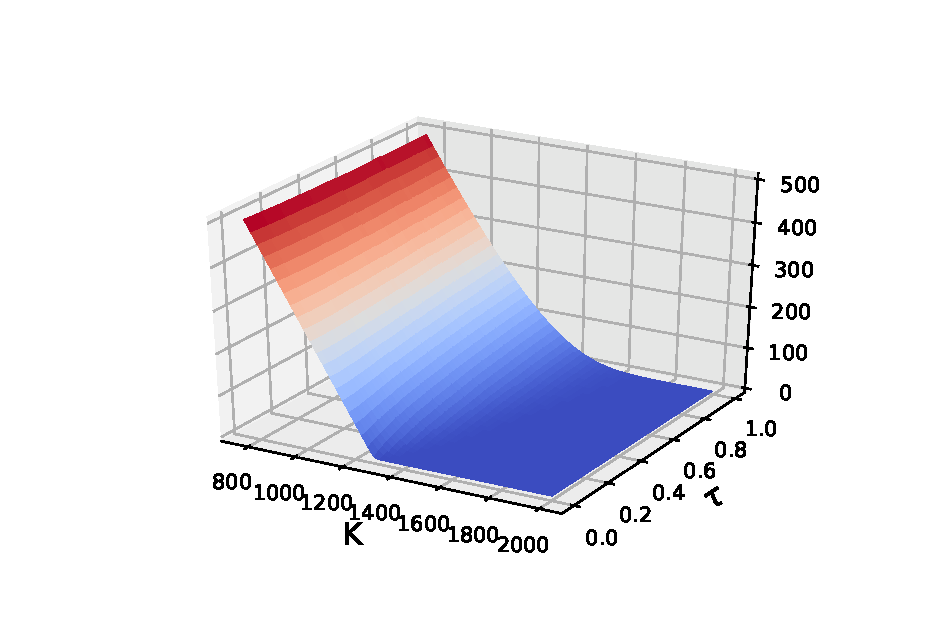
\includegraphics[width=0.60\textwidth]{../../figures/Price}
\caption{An Arbitrage-Free Surface}
\end{figure}
\end{itemize}


\end{frame}






\subsection{Data-Driven Sequential Learning Framework For Total Risk Hedging}
\begin{frame}{Local Versus Total Risk Hedging}
The {\em discrete total hedging risk} is the summation of the {\em discrete local hedging risk} evaluated at discrete rebalancing time $\{t_0,t_1,\dots,t_{N_{rb}-1}\}$. 
\[
    \text{Risk}^{total}_{t_0}=\sum_{j=0}^{N_{rb}-1}\left\{ \Delta \Smkt_{t_j} \delta_{t_j} -\Delta \Vmkt_{t_j} \right\}=\sum_{j=0}^{N_{rb}-1}\text{Risk}^{local}_{t_j}
\]
As a consequence, building a model reducing the discrete local hedging risk will reduce the discrete total hedging risk as well. 
\begin{figure}[htp!]
	\centering
	\subfigure[]{
		\includegraphics[width=0.30\textwidth]{../../figures/LocalVersusTotalNTM.pdf}}
	\subfigure[]{
		\includegraphics[width=0.30\textwidth]{../../figures/LocalVersusTotalITM.pdf}}
	\subfigure[]{
		\includegraphics[width=0.30\textwidth]{../../figures/LocalVersusTotalOTM.pdf}}
\caption{Weekly Hedging Put Option}
\end{figure}
\end{frame}

\section{Conclusion and Future Works}
\begin{frame}{Conclusion}
Data-driven  hedging model shows potential for improved performance over classical methods:
\begin{itemize}
\item The kernel model $\DKLs$ improves  local risk hedging performance over the classical parametric hedging strategy.
\item The sequential model $\model$ significantly outperforms MV, SABR-Bartlett, and kernel model $\DKLs$ in local risk hedging.
\item  The  extension to multi-step total risk hedging scenarios often outperforms SABR-Bartlett, and Black-Scholes in total risk hedging measurement. 
\item The data-driven local risk hedging model remains competitive in terms of total risk measurements.
\end{itemize}
\end{frame}
\begin{frame}{Future Works}
\begin{itemize}
	\item  Generate  hedging risk scenarios (e.g., using GAN)  to build more complex model for hedging.
	\item  Incorporate transaction cost, allow flexible rebalancing frequency, extend to hedge more complex derivatives, etc.
	\item  Extension to calculate implicit exposure across different assets. 
\end{itemize}
\end{frame}

\begin{frame}{Contribution}
\begin{itemize}
\item Ke Nian, Thomas F Coleman, and Yuying Li. Learning minimum variance discrete hedg-
ing directly from the market. Quantitative Finance, 18(7): 1115–1128, 2018.
\item Ke Nian, Thomas F Coleman, and Yuying Li. Learning sequential option hedging models
from market data. Journal of Banking \& Finance, 133:106-277, 2021.
\item Ke Nian, Thomas F Coleman, and Yuying Li. Learning sequential total hedging models
from market data. In Preparation, 2023.
\end{itemize}
\end{frame}

\begin{frame}{Q \& A}
\LARGE
\begin{quote}
	\alert{Thank you very much!}\\
	\hspace{8ex} Any Questions?
\end{quote}
\end{frame}

\end{document}